\documentclass[]{beamer}
\usepackage[T1]{fontenc}
\usepackage[utf8]{inputenc}
\usepackage{lmodern}
\usepackage[italian]{babel}
\usepackage{mathrsfs}
\usepackage{cancel}

\title{La crisi della fisica classica e l'ipotesi quantistica}
\author{\texorpdfstring{Mattia Cozzi\newline\href{mailto:cozzimattia@gmail.com}{\texttt{cozzimattia@gmail.com}}}{Mattia Cozzi}}
\date{a.s.~2023/2024}

%\documentclass[handout]{beamer}     %usare questa classe per generare l'handout
%\usepackage{pgfpages}   %per mostrare più quadri nella stessa pagina
%\pgfpagesuselayout{4 on 1}[a4paper,border shrink=5mm,landscape]
\usetheme{Singapore}
%\useoutertheme[left]{sidebar} %elementi intorno alle diapositive
\setbeamercovered{dynamic} %modifica l'aspetto del testo grigetto delle diapositive future. Argomenti: invisible/transparent/dynamic
\usecolortheme{orchid}
%COLORE PRINCIPALE
% \definecolor{marroncino}{RGB}{156, 26, 0} % UBC Blue (primary)
% \setbeamercolor{structure}{fg=marroncino} % itemize, enumerate, etc


\theoremstyle{plain}
\newtheorem{teorema}{Teorema}

\usepackage{tikz}
\usepackage{circuitikz}

\usepackage{pgf,pgfplots,graphicx}
\usetikzlibrary{angles,quotes,arrows,shapes,decorations.markings}
\pgfplotsset{compat=1.15}
\usepgfplotslibrary{units,fillbetween} % to add units easily to axis

\newcommand{\fem}{f_{em}}

\def\angolo[#1](#2)(#3:#4:#5)% Syntax: [draw options] (center) (initial angle:final angle:radius)
    { \draw[#1] ($(#2)+({#5*cos(#3)},{#5*sin(#3)})$) arc (#3:#4:#5); }


\newcommand<>{\xxcancel}[1]{\alt#2{\xcancel{#1}\vphantom{#1}}{#1}}

\begin{document}

\begin{frame}
  \titlepage
\end{frame}





\begin{frame}
\frametitle{Contenuti}
\tableofcontents
\end{frame}


\section{Corpo nero}

\begin{frame}
\frametitle{Cosa è un corpo nero}
\begin{block}{Definizione}
  Un corpo nero è un oggetto ideale che assorbe tutta la radiazione elettromagnetica (cioè le onde elettromagnetiche) incidente senza rifletterla.
\end{block}\pause

~

Gli oggetti quotidiani non possiedono \emph{esattamente} questa proprietà e sono detti \alert{corpi grigi}.\pause

~

Un oggetto reale che si avvicina al corpo nero è la \emph{grafite}, che assorbe il $ 97\% $ della radiazione incidente.
\end{frame}


\begin{frame}
\frametitle{Assorbimento e irradiamento (1)}
Un corpo nero:

\begin{enumerate}
  \item assorbe energia e raggiunge una certa temperatura;\pause
  \item emette energia sotto forma di \emph{onde elettromagnetiche} in \alert<2>{tutte le lunghezze d'onda}.\pause
\end{enumerate}

~

Si dimostra sperimentalmente che \alert<3>{la ripartizione dell'energia nelle diverse lunghezze d'onda dipende unicamente dalla temperatura del corpo}.
\end{frame}


\begin{frame}
\frametitle{Assorbimento e irradiamento (2)}
A temperature maggiori corrispondono picchi di emissione di onde con $ \lambda $ minore.\pause

~

Oggetti a temperature maggiori emetteranno più luce di colore blu, oggetti più freddi emetteranno più luce di colore rosso:

\begin{center}
$ \textcolor{blue}{\lambda_{blu}} < \textcolor{red}{\lambda_{rosso}} $
\end{center}

\visible<2>{\begin{figure}
  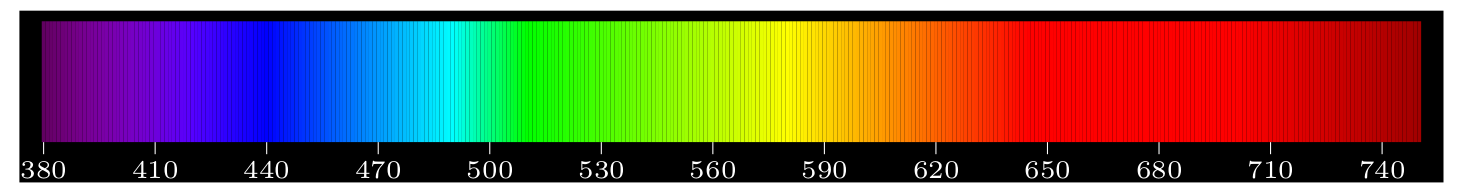
\includegraphics[width=\columnwidth]{img/spettrolum.png}
  {\small $ \lambda \, [nm]$}
\end{figure}}

\end{frame}


\begin{frame}
\frametitle{Grafico dell'irradiamento}
Rappresentiamo la \alert<1>{curva sperimentale} dell'energia emessa per unità di superficie in funzione della lunghezza d'onda $ \lambda $.
\begin{figure}
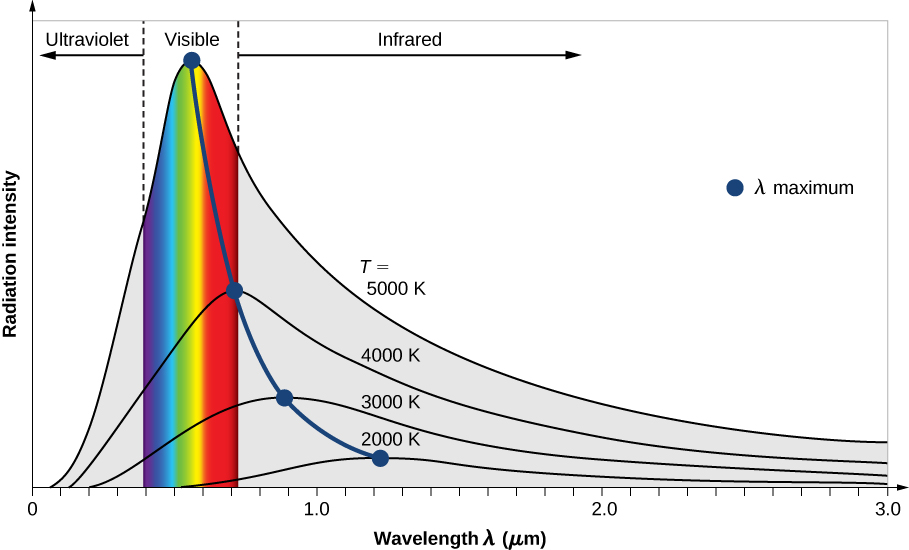
\includegraphics[width=.85\columnwidth]{img/corponero.jpg}
\end{figure}\pause
L'area sottesa dal grafico fornisce l'energia totale emessa.
\end{frame}

\begin{frame}
\frametitle{Emissione di onde e temperatura}

\begin{figure}
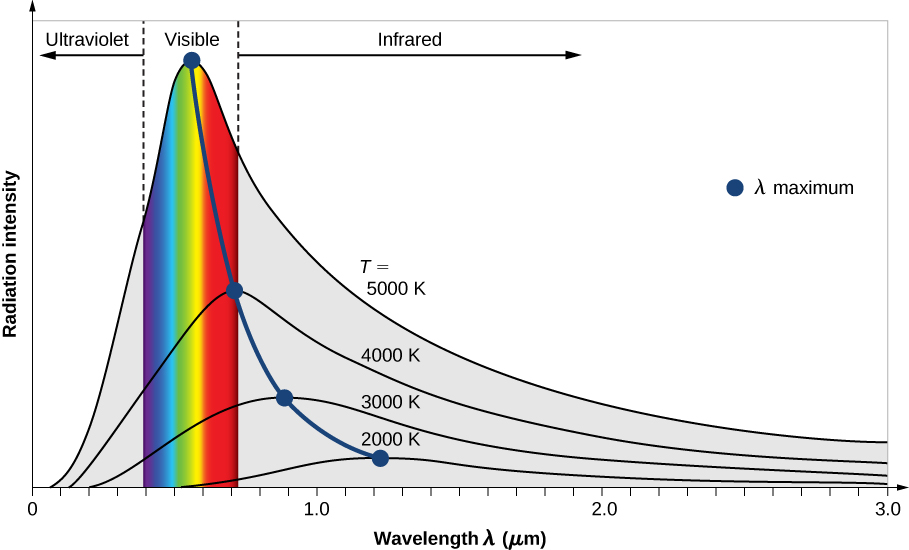
\includegraphics[width=.65\columnwidth]{img/corponero.jpg}
\end{figure}
\pause
All'aumentare di $ T $, il picco di emissioni si sposta sempre più nel visibile, diventando prima rosso, poi arancione, giallo, bianco, blu.\pause

~

Quando vediamo il corpo blu, buona parte della radiazione è emessa nell'ultravioletto.
\end{frame}



\begin{frame}
\frametitle{Legge di Wien}
La lunghezza d'onda del picco di emissioni può essere calcolata con una \alert<1>{legge sperimentale}, la legge di spostamento di Wien:
\begin{center}
  \colorbox{blue!30}{$ \displaystyle \lambda_{max} = \dfrac{2,90 \times 10^{-3} \, m \cdot K}{T} $}
\end{center}
\end{frame}



\begin{frame}
\frametitle{Corpi ideali e corpi reali}
A temperatura ambiente, i corpi neri emettono di fatto solo radiazione infrarossa.
\begin{columns}
\begin{column}{0.45\textwidth}
\begin{figure}
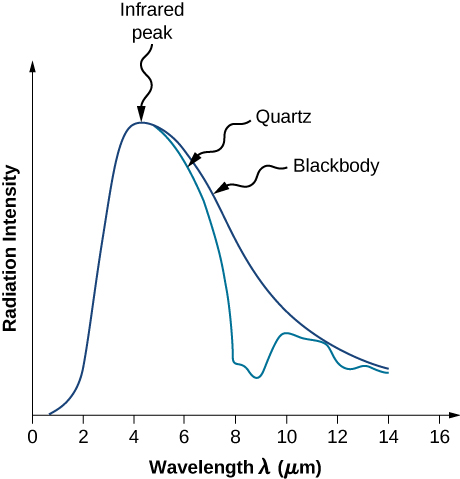
\includegraphics[width=\columnwidth]{img/corponero2.jpg}
\end{figure}
\end{column}

\begin{column}{0.45\textwidth}
\begin{figure}
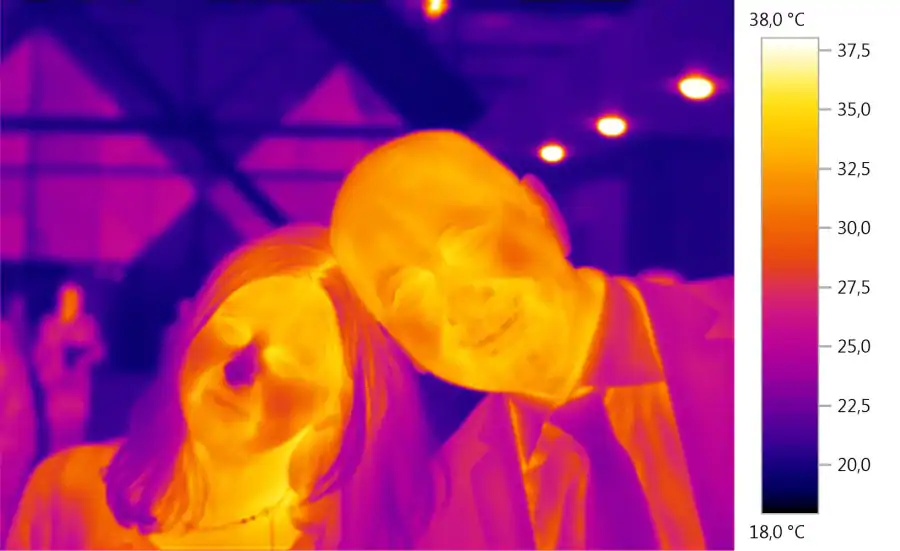
\includegraphics[width=\columnwidth]{img/corponero3.png}
\end{figure}
\end{column}
\end{columns}

\end{frame}




\begin{frame}
\frametitle{Previsione classica: un problema (grosso)}
Si tentò di spiegare le curve sperimentali \alert{partendo dalla teoria elettromagnetica e dalla termodinamica}.\pause
\visible<2>{\begin{figure}
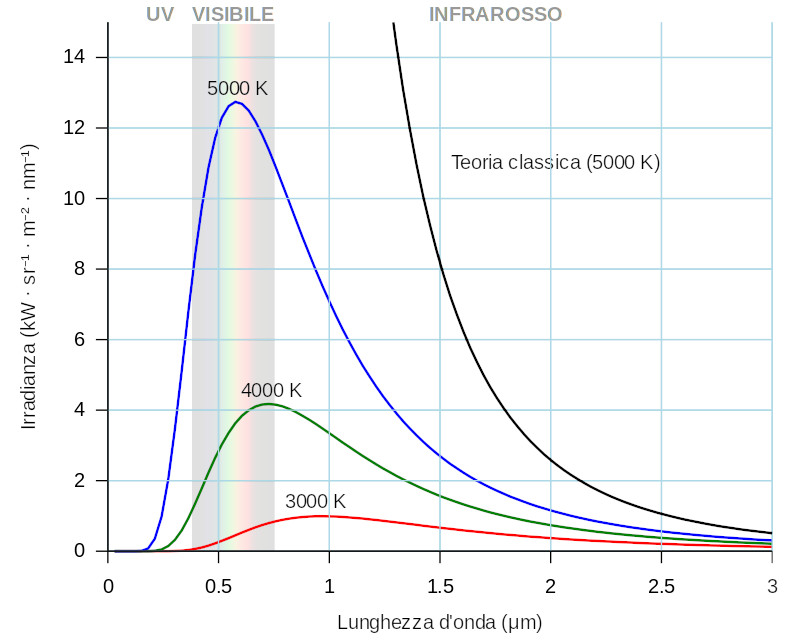
\includegraphics[width=.6\columnwidth]{img/catastrofe.jpg}
\end{figure}}
L'approccio classico forniva la previsione mostrata nel grafico.
\end{frame}


\begin{frame}
\frametitle{La catastrofe ultravioletta}
\begin{columns}
\begin{column}{0.55\textwidth}
\begin{figure}
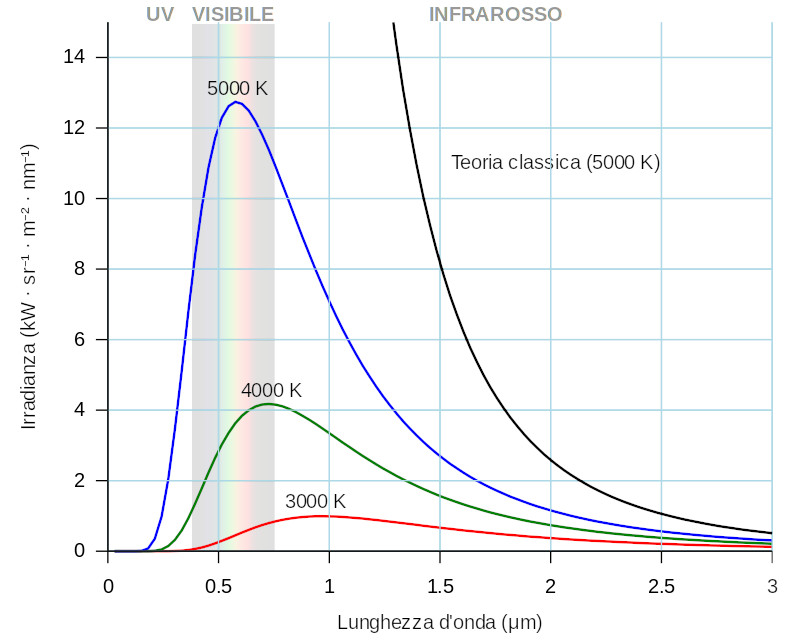
\includegraphics[width=\columnwidth]{img/catastrofe.jpg}
\end{figure}
\end{column}

\begin{column}{0.4\textwidth}
La teoria classica poteva (approssimativamente) essere adeguata nella zona dell'infrarosso, ma spostandoci verso l'ultravioletto vediamo come la curva teorica sottenda un'area infinita, in totale \alert{violazione del principio di conservazione dell'energia}.
\end{column}
\end{columns}\pause

~

~

L'area sottesa dalla curva della previsione classica è infinita!
\end{frame}

\section{Planck}

\begin{frame}
\frametitle{L'ipotesi di Planck (1900)}
Nel 1900 Max Planck scoprì come modificare la teoria della radiazione elettromagnetica per ottenere una previsione teorica in accordo coi dati sperimentali.\pause

~

In precedenza si era assunto che lo scambio di energia tra gli atomi del corpo nero e le onde elettromagnetiche avvenisse in modo \alert<2>{continuo}, con scambi di energia qualsiasi per qualsiasi lunghezza d'onda/frequenza.
\end{frame}

\begin{frame}
\frametitle{L'ipotesi di Planck (1900)}
Planck propone una ipotesi \emph{ad hoc} per accordare la teoria con i dati sperimentali (su di lui gravavano anche pressioni politiche da parte del governo tedesco).\pause

~

\begin{quote}
Fu un atto di disperazione. Avevo già lottato per sei anni con il problema del corpo nero. Sapevo che il problema era fondamentale e ne conoscevo la legge; una spiegazione teorica doveva trovarsi a qualunque costo, salvo l'inviolabilità delle leggi della termodinamica.
\end{quote}

\begin{center}
\href{https://claesjohnsonmathscience.wordpress.com/article/the-desperation-of-planck-yvfu3xg7d7wt-79/}{\beamergotobutton{Lettura: The Desperation of Planck}}
\end{center}
\end{frame}


\begin{frame}
\frametitle{L'ipotesi di Planck (1900)}
\begin{block}{Ipotesi quantistica}
Lo scambio di energia tra il corpo nero e le onde elettromagnetiche avviene attraverso il trasferimento di \alert{quanti} di energia, ognuno di valore:
\begin{center}
\colorbox{blue!30}{$ E = hf $}
\end{center}
$ h $ = costante di Planck = $ 6,627 \times 10^{-34} \, J\cdot s $ 
\end{block}\pause

~

L'energia totale scambiata (emessa) deve essere un \alert{multiplo intero} di questa quantità:
\begin{center}
$ E_{tot} = nhf $
\end{center}
\end{frame}


\begin{frame}
\frametitle{Fisica quantistica (1)}
Nonostante le reticenze iniziali dello stesso Planck a considerare tale ipotesi in corrispondenza con un reale fenomeno fisico, questo è \alert{l'inizio della Fisica quantistica}.

~

\begin{quote}
 If $ E $ [is] considered to be [a] continuously divisible quantity, this distribution is possible in infinitely many ways. We consider, however -- this is the most essential point of the whole calculation -- $ E $ to be composed of a very definite number of equal parts and use thereto the constant of nature $ h $.
\end{quote}
\end{frame}







\begin{frame}
\frametitle{Esercizio}
\begin{exampleblock}{``Pacchetti di energia''}
\small{
  Una quantità di $ 0,50 \, kg $ di acqua è investita dalla radiazione solare e la sua temperatura aumenta di $ 1,0 \, K $. Considera la radiazione solare monocromatica, con una lunghezza d'onda pari al massimo della distribuzione spettrale ed emessa da una sorgente alla temperatura di $ 5,8 \times 10^{3} \, K $.
  
  Stima il numero minimo di ``pacchetti di energia'' giunti con la radiazione solare.\hspace*{\fill}[$ 5,3 \times 10^{21} $]
  }
\end{exampleblock}
\end{frame}




\begin{frame}
\frametitle{Fisica quantistica (2)}
Negli anni successivi diversi esperimenti e proposte teoriche per spiegarli daranno sempre maggior forza all'ipotesi quantistica.\pause

~

\begin{itemize}
  \item effetto fotoelettrico (1902) e sua spiegazione (1905);\\
     $ \Rightarrow  $ emissione di elettroni da parte di una lastra metallica\pause
  \item esperimento di Millikan (1909);\\
     $ \Rightarrow  $ misura della carica dell'elettrone\pause
  \item esperimento di Geiger e Marsden (1909) e atomo di Rutherford (1911);\\
    $ \Rightarrow  $ scoperta del nucleo atomico\pause
  \item modello atomico di Bohr (1913);\\
    $ \Rightarrow  $ modello atomico quantistico\pause
  \item esperimento di Franck e Hertz (1914);\pause
  \item effetto Compton (1923). 
\end{itemize}
\end{frame}




\section{Effetto fotoelettrico}

\begin{frame}
\frametitle{L'esperimento di Lenard (1902)}

\begin{figure}
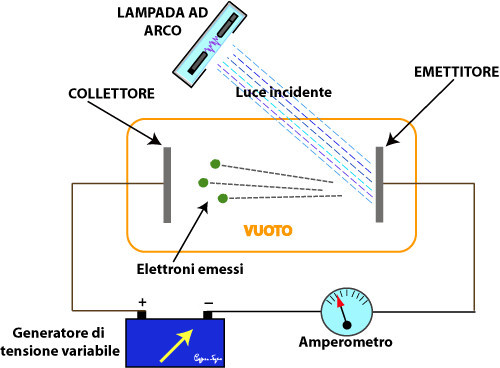
\includegraphics[width=.6\columnwidth]{img/lenard1.jpg}
\end{figure}\pause

Se il collettore ha potenziale positivo, gli elettroni sono ``raccolti'' e si ha una corrente.\pause

~

Se \emph{tutti} gli elettroni sono raccolti, si ha la \emph{corrente  limite}.

\end{frame}


\begin{frame}
\frametitle{L'esperimento di Lenard (1902)}

\begin{figure}
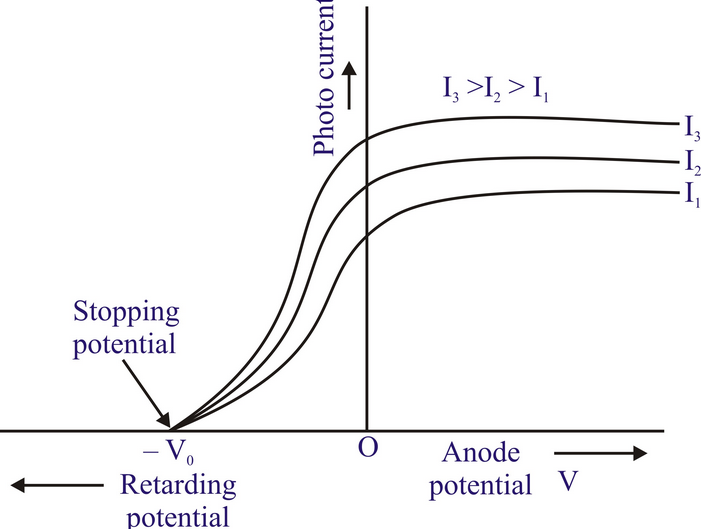
\includegraphics[width=.4\columnwidth]{img/correntelimite.png}
\end{figure}

Il valore della corrente limite dipende dall'irradiamento subito dal metallo.

\begin{center}
$ I = \dfrac{\Delta E}{A \cdot t} \, \left[ \dfrac{W}{m^2} \right] $
\end{center}

\end{frame}


\begin{frame}
\frametitle{L'esperimento di Lenard (1902)}
Proviamo a invertire la polarità di tra collettore ed emettitore.

~

\begin{figure}
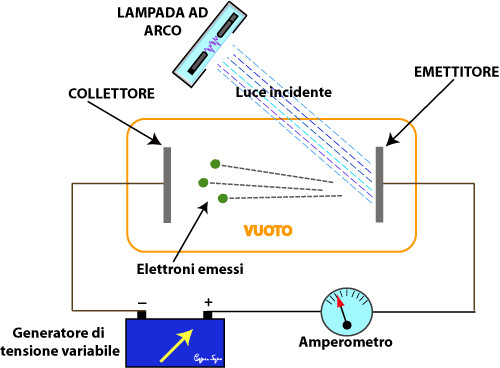
\includegraphics[width=.6\columnwidth]{img/lenard2.jpg}
\end{figure}\pause
Gli elettroni vengono ``frenati'' dalla differenza di potenziale e la corrente diminuisce.

\end{frame}


\begin{frame}
\frametitle{L'esperimento di Lenard (1902)}
\begin{figure}
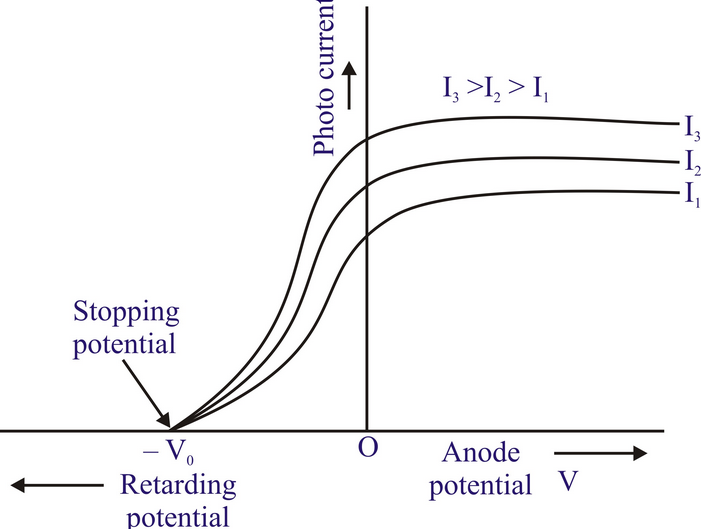
\includegraphics[width=.4\columnwidth]{img/correntelimite.png}
\end{figure}\pause
Aumentando sempre di più la differenza di potenziale, possiamo annullare la corrente. 

~

Abbiamo raggiunto il \emph{potenziale di arresto} $ -\Delta V_a $.

~

Notiamo che \alert{il potenziale di arresto non dipende dall'irradiamento}.

\end{frame}

\begin{frame}
\frametitle{Energia cinetica}
Ricorda: una carica $ q $, sottoposta ad una differenza di potenziale $ \Delta V $, riceve un'energia potenziale $ U = q \Delta V $.\pause

~

Quando sono emessi, gli elettroni hanno una certa energia cinetica $ K_{max} $.\pause

~

Quando si fermano, hanno convertito tutta la loro energia cinetica in energia potenziale $ U = (-e)(-\Delta V_a) = e\Delta V_a $.
\end{frame}




\begin{frame}
\frametitle{Un problema (1)}
Per la conservazione dell'energia:
\begin{center}
$ U = K_{max}~~~~~\Longrightarrow~~~~~ $\colorbox{blue!30}{$ K_{max} = e\Delta V_a $}
\end{center}\pause
Possiamo quindi, conoscendo $ \Delta V_a $, calcolare $ K_{max} $.\pause

~

Poiché $ \Delta V_a $ non dipende dall'irradiamento, anche \alert<3>{$ K_{max} $ non dipende dall'irradiamento}.\pause

~

Questo \alert<4>{pone un problema per l'elettromagnetismo classico}, secondo cui le onde e.m.~forniscono energia agli $ e $ in modo da farli emettere dalla piastra (\emph{energia di estrazione}).\pause

~

Se aumenta l'irradiamento, aumenta l'energia che colpisce il metallo e \alert<4>{dovrebbe aumentare l'energia cinetica degli $ e $ emessi}.
\end{frame}

\begin{frame}
\frametitle{Un problema (2)}
Secondo i dati sperimentali, \alert{$ K_{max} $ dipende dalla frequenza della radiazione incidente} (oltre una frequenza di soglia $ f_{min} $).

\begin{figure}
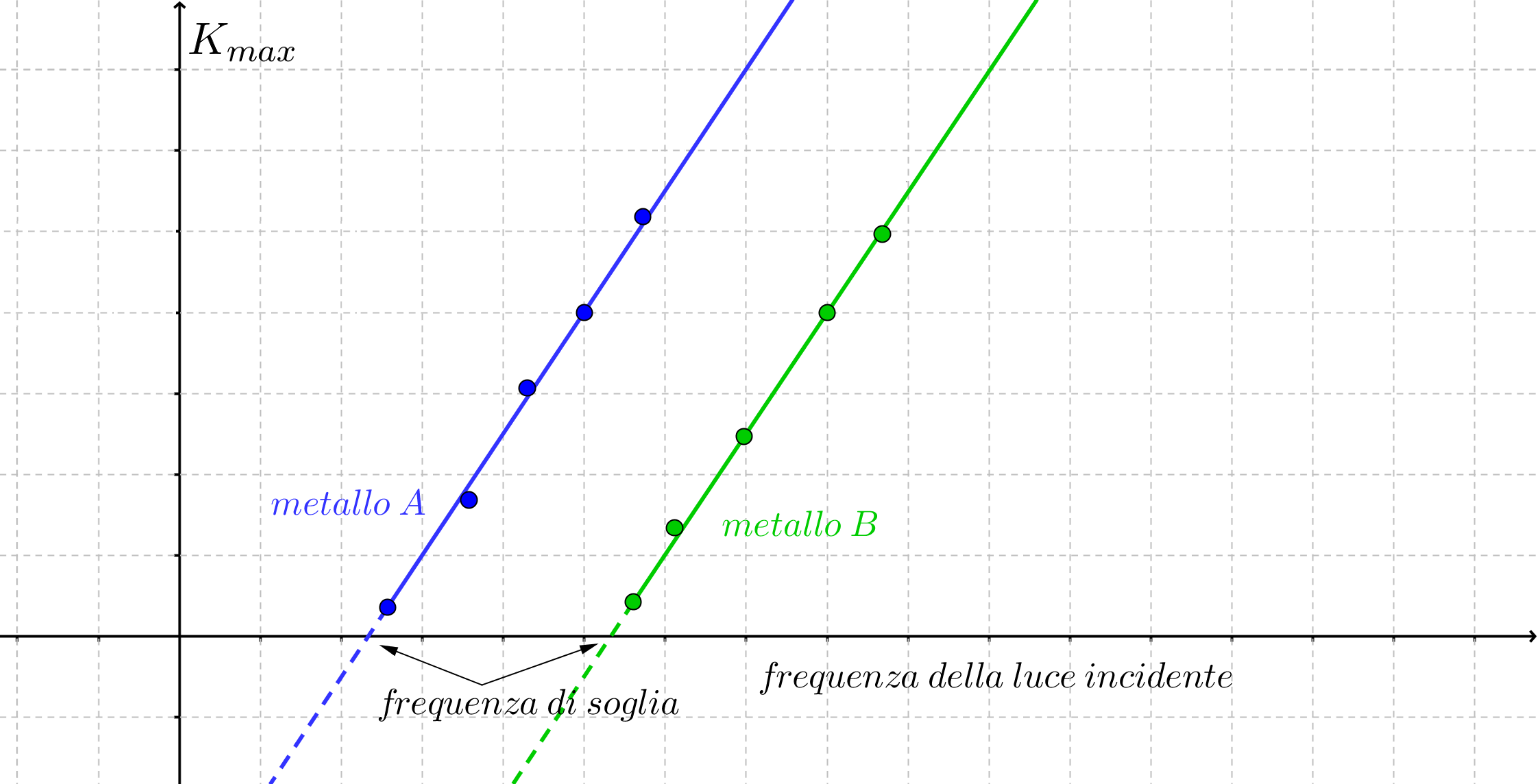
\includegraphics[width=.8\columnwidth]{img/fotoelettrico1.png}
\end{figure}
\pause

~

Secondo la teoria classica, ogni onda può estrarre elettroni, finché fornisce un'energia maggiore di $ L_e $ (lavoro di estrazione).


\end{frame}

\begin{frame}
\frametitle{Einstein e Planck}
Per spiegare questi risultati sperimentali, Einstein ``prende sul serio'' l'ipotesi di Planck (1900), secondo cui:
\begin{block}{Postulato di Planck}
Gli scambi di energia avvengono attraverso lo scambio di \alert{quanti di energia}, ognuno di valore:
\begin{center}
\colorbox{blue!30}{$ E = hf $}
\end{center}
$ h = 6,627 \times 10^{-34} \, J \cdot s $
\end{block}\pause

~

Einstein pubblica i suoi risultati nel 1905 (\emph{annus mirabilis}), chiamando i quanti del campo elettromagnetico \alert{fotoni}.

\end{frame}


\begin{frame}
\frametitle{Spiegazione dell'effetto fotoelettrico (1)}
L'idea di Einstein è che \alert<1>{se l'energia $ hf $ di un fotone è superiore a $ L_e $, allora si ha l'emissione dell'elettrone}. \pause

~

Esiste quindi una frequenza minima per l'emissione (quando \alert<2>{$ hf=L_e $}):
\begin{center}
$ f_{min} = \dfrac{L_e}{h} $
\end{center}\pause

Il resto dell'energia rimane all'elettrone come \alert<3>{energia cinetica}.
\begin{center}
\colorbox{blue!30}{$ K_{max} = hf - L_e $}
\end{center}
\end{frame}



\begin{frame}
\frametitle{Spiegazione dell'effetto fotoelettrico (2)}

\begin{center}
\colorbox{blue!30}{$ K_{max} = hf - L_e $}
\end{center}

\begin{figure}
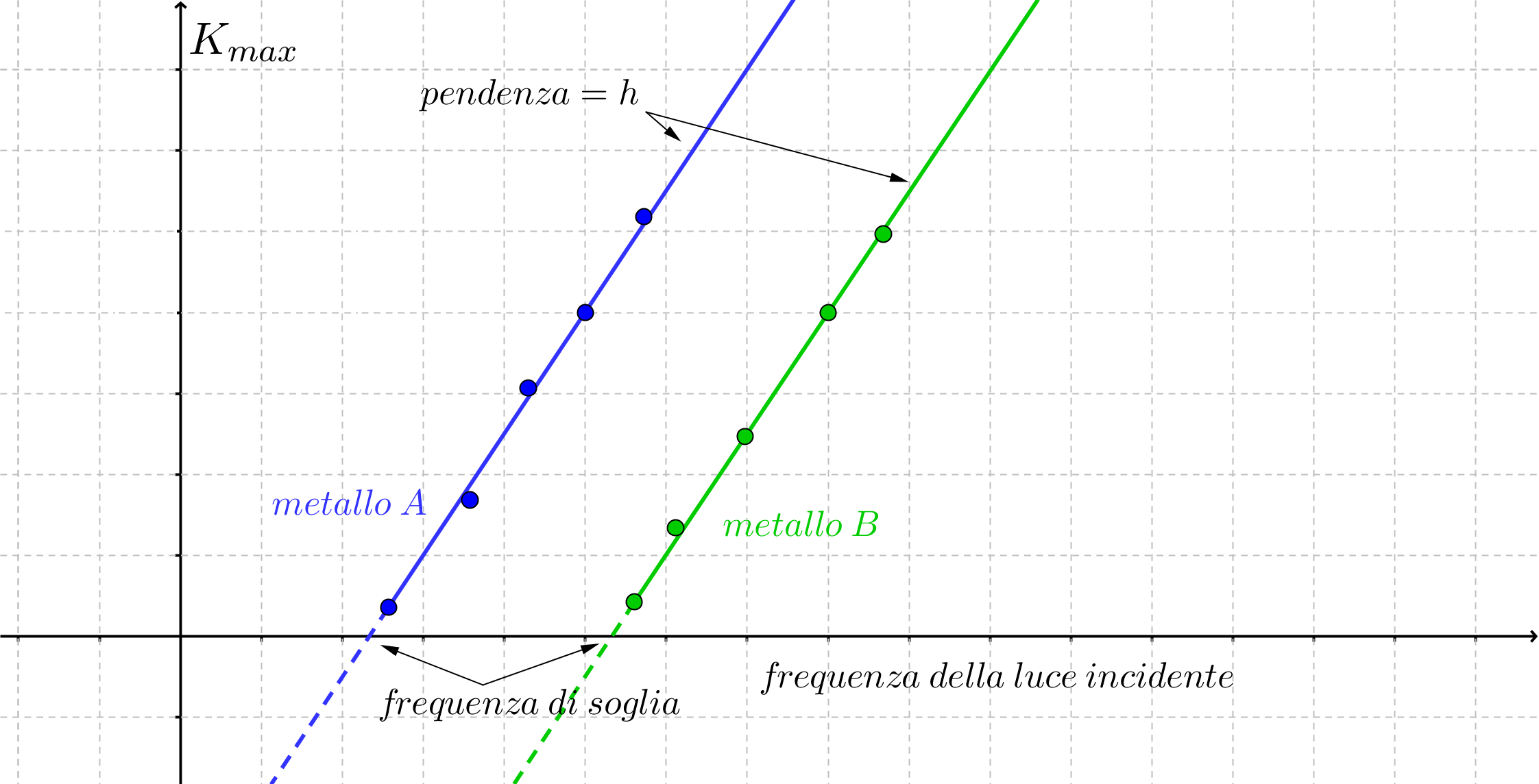
\includegraphics[width=.9\columnwidth]{img/fotoelettrico2.png}
\end{figure}
\end{frame}





\begin{frame}
\frametitle{Esercizio}
\begin{exampleblock}{Lavoro di estrazione}
\small{
Su una superficie incide una radiazione con lunghezza d'onda $ \lambda \, 330 nm $. Gli elettroni estratti possiedono un'energia di $ 0,200 \, eV $.

Ricordando che $ 1 \, eV = 1,60 \times 10^{-19} \, J $, calcola il lavoro di estrazione relativo a quella superficie.\hspace*{\fill}[$ 5,71 \times 10^{-19} \, J $]
  }
\end{exampleblock}
\end{frame}



\section{Effetto Compton}

\begin{frame}
\frametitle{Fotoni?}
Per molti anni l'idea della luce composta da \alert<1>{fotoni} non fu accettata (nemmeno dallo stesso Planck), poiché pareva ovvio che la luce, presentando il fenomeno dell'interferenza, dovesse essere un'onda.\pause

~

Questa reticenza fu finalmente superata nel 1923 grazie al lavoro di Arthur Compton, che spiegò l'effetto che porta il suo nome.
\end{frame}


\begin{frame}
\frametitle{Situazione sperimentale}
Vengono inviati dei raggi X ($ \lambda = 7,09 \times 10^{-11} \, m $) su un bersaglio di grafite.

~

Una parte dei raggi attraversa invariata il bersaglio, una parte viene diffusa con diversi angoli $ \varphi $.

\begin{figure}
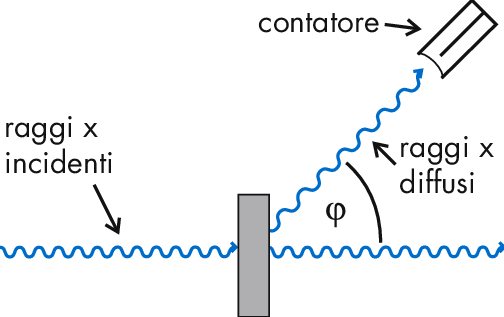
\includegraphics[width=.55\columnwidth]{img/compton.png}
\end{figure}
\end{frame}

\begin{frame}
\frametitle{Previsione e spiegazione classica}
La fisica classica spiegava questo effetto ipotizzando che:
\begin{enumerate}
  \item i raggi X ``colpiscono'' gli elettroni della grafite, facendoli oscillare;\pause
  \item la frequenza di oscillazione degli elettroni è la stessa dei raggi X;\pause
  \item cariche oscillanti emettono onde elettromagnetiche;\pause
  \item la frequenza delle onde emesse è la stessa con cui oscillano gli elettroni.
\end{enumerate}
\end{frame}



\begin{frame}
\frametitle{Risultati sperimentali}
Si ha un picco di radiazioni diffuse per $ \varphi = 90^{\circ} $.
\begin{columns}
\begin{column}{0.5\textwidth}
\begin{figure}
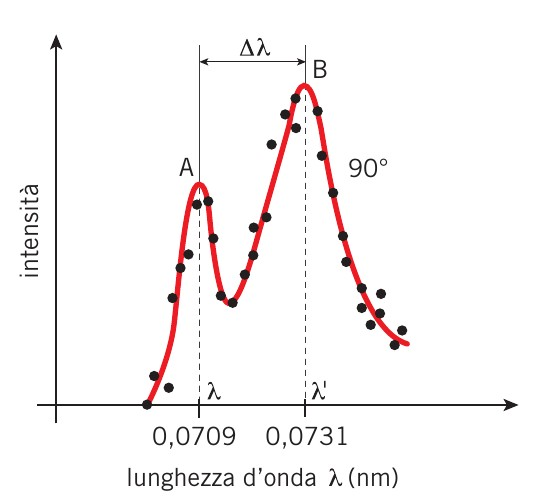
\includegraphics[width=\columnwidth]{img/compton2.jpg}
\end{figure}
\end{column}
\begin{column}{0.4\textwidth}
Il problema nasce dalla constatazione che \alert{la radiazione diffusa ha lunghezza d'onda diversa da quella della radiazione incidente}:
\begin{center}
$ \lambda = 7,09 \times 10^{-11} \, m $

~

$ \lambda' = 7,31 \times 10^{-11} \, m $
\end{center}
\end{column}
\end{columns}\pause

~

Anche questo fenomeno non è spiegabile con la teoria classica.
\end{frame}


\begin{frame}
\frametitle{La spiegazione di Compton (1)}
Compton accetta l'idea dei fotoni e propone:
\begin{block}{Interazione fotone-elettrone}
Le onde elettromagnetiche sono composte di fotoni $ \gamma $ che interagiscono con gli elettroni come particelle durante un urto elastico.
\end{block}\pause

~

Sappiamo che:
\begin{center}
$ E_\gamma = hf = \dfrac{hc}{\lambda} $~~~~~~~~e~~~~~~~~$ p_\gamma = \dfrac{E\gamma}{c} = \dfrac{h}{\lambda} $
\end{center}\pause

~

Colpendo un elettrone, \alert{il fotone trasferisce ad esso una parte della sua energia (cinetica) e della sua quantità di moto}.
\end{frame}



\begin{frame}
\frametitle{La spiegazione di Compton (2)}
\begin{center}
$ E_\gamma = \dfrac{hc}{\lambda} $~~~~~~~~~~~~~~~~$ p_\gamma = \dfrac{h}{\lambda} $
\end{center}

~

Se $ E_\gamma $ e $ p_\gamma $ diminuiscono, $ \lambda $ deve necessariamente aumentare e pertanto \alert{la lunghezza d'onda $ \lambda' $ dei raggi diffusi è maggiore di $ \lambda $}.\pause

~

\visible<2>{\begin{figure}
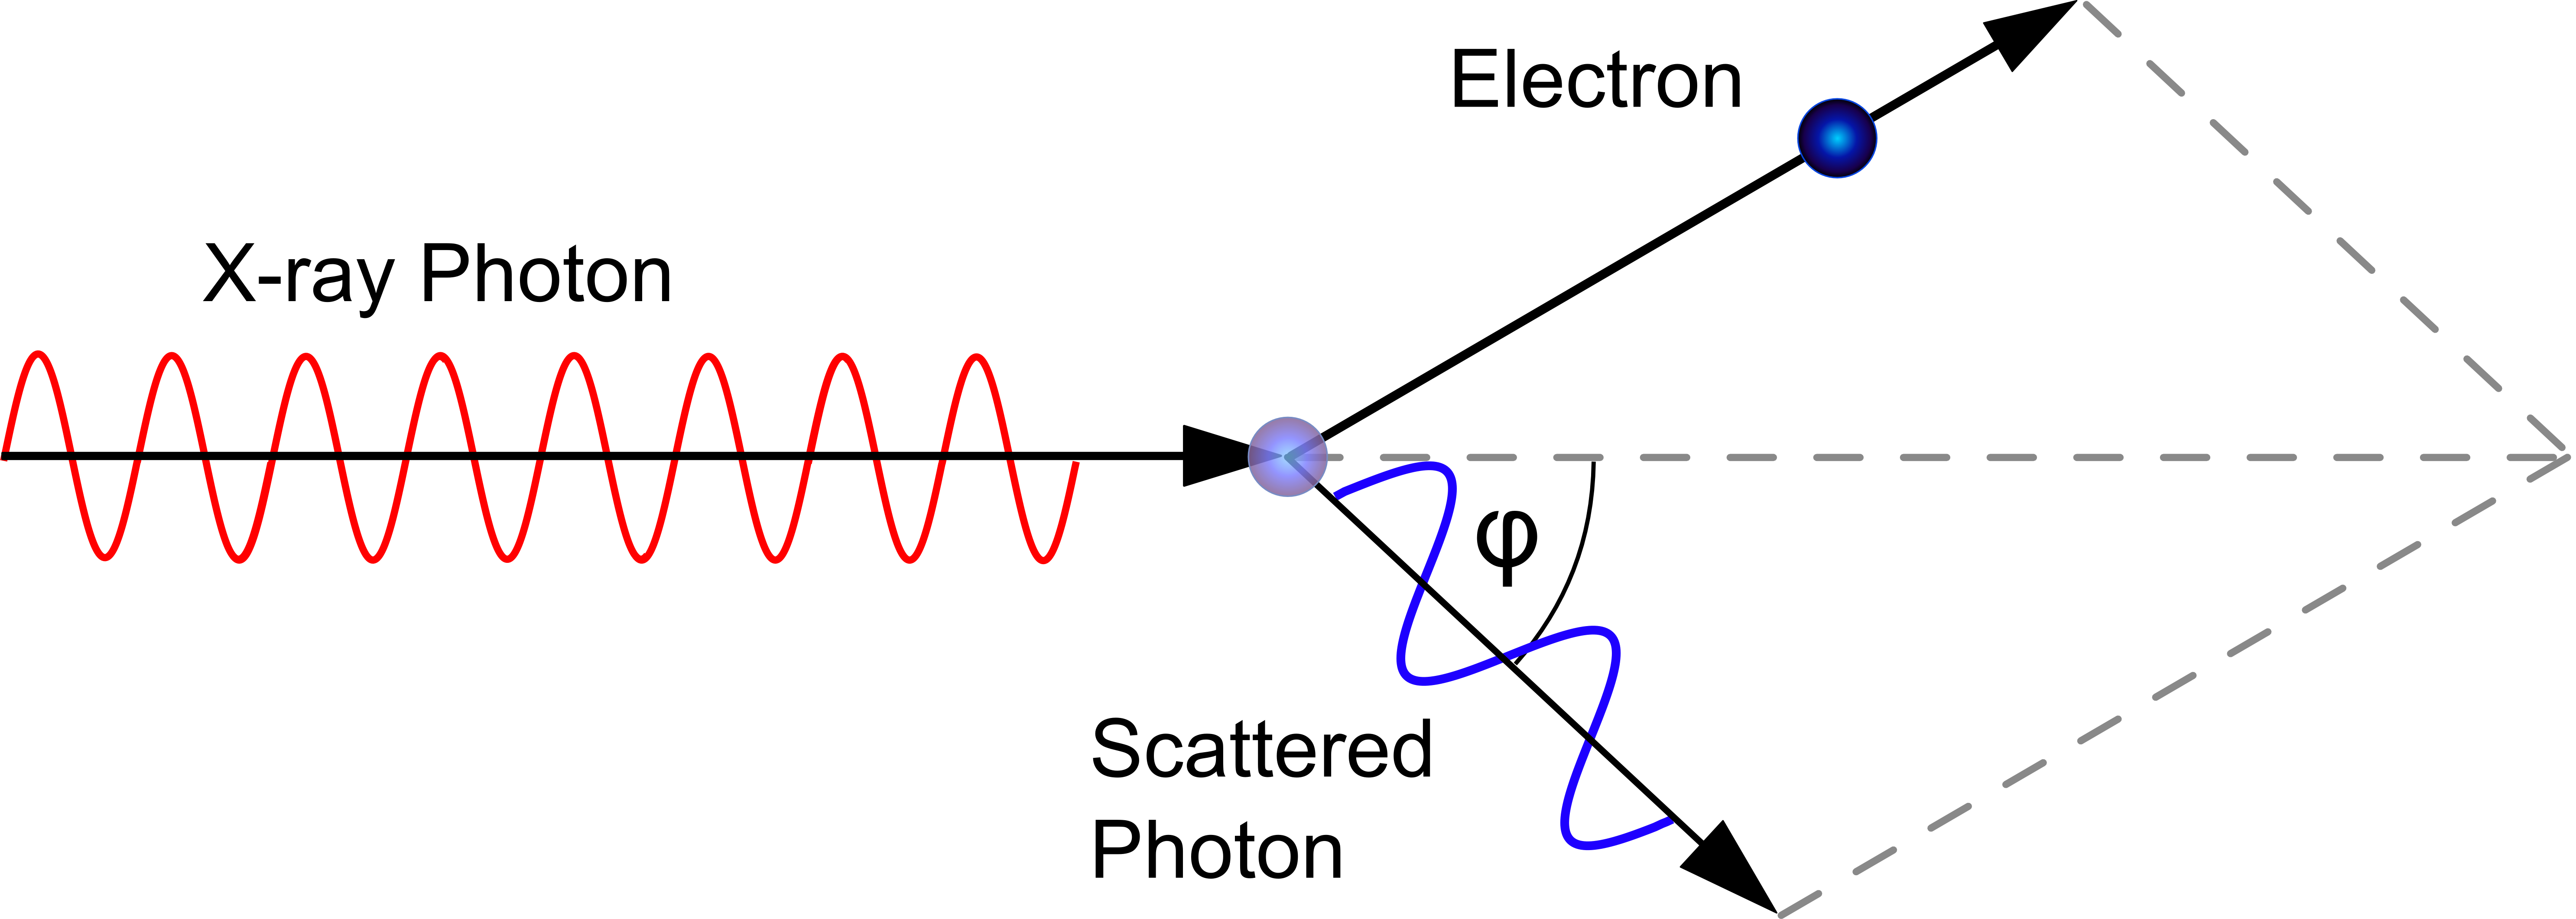
\includegraphics[width=.85\columnwidth]{img/compton3.png}
\end{figure}}
\end{frame}




\section{Spettro}


\begin{frame}
\frametitle{Generazione di uno spettro}

\begin{columns}
\begin{column}{0.5\textwidth}
\visible<1->{Se un gas monoatomico è portato ad alta temperatura o attraversato da corrente elettrica esso \emph<1>{emette luce}.}

~

\visible<2->{Con un prisma, otteniamo uno \alert<2->{spettro di emissione}.}
\end{column}
\begin{column}{0.5\textwidth}
\visible<3->{Possiamo inoltre far \emph<3>{attraversare il gas da luce bianca}, per poi scomporre con un prisma la luce ottenuta.}

~

\visible<4->{In questo caso abbiamo uno \alert<4->{spettro di assorbimento}.}
\end{column}
\end{columns}

\visible<2->{\begin{figure}
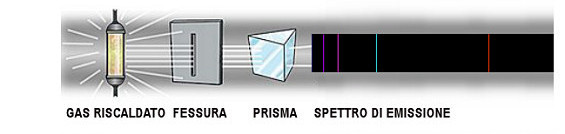
\includegraphics[width=.6\columnwidth]{img/spettro1.jpg}
\end{figure}}

\visible<4->{\begin{figure}
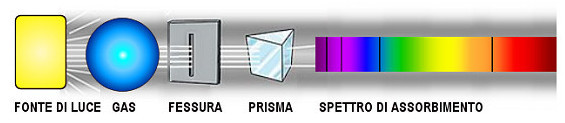
\includegraphics[width=.6\columnwidth]{img/spettro2.jpg}
\end{figure}}
\end{frame}

\begin{frame}
\frametitle{Spettri dell'atomo di idrogeno}
\begin{figure}
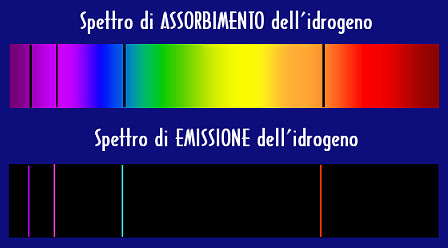
\includegraphics[width=.7\columnwidth]{img/spettriidrogeno.jpg}
\end{figure}\pause
Notiamo che:
\begin{itemize}
  \item l'idrogeno monoatomico può assorbire ed emettere solo e soltanto alcune lunghezze d'onda;\pause
  \item le linee sono più dense per lunghezze d'onda minori.
\end{itemize}
\end{frame}



\begin{frame}
\frametitle{Spettri di altri elementi e molecole}
\begin{figure}
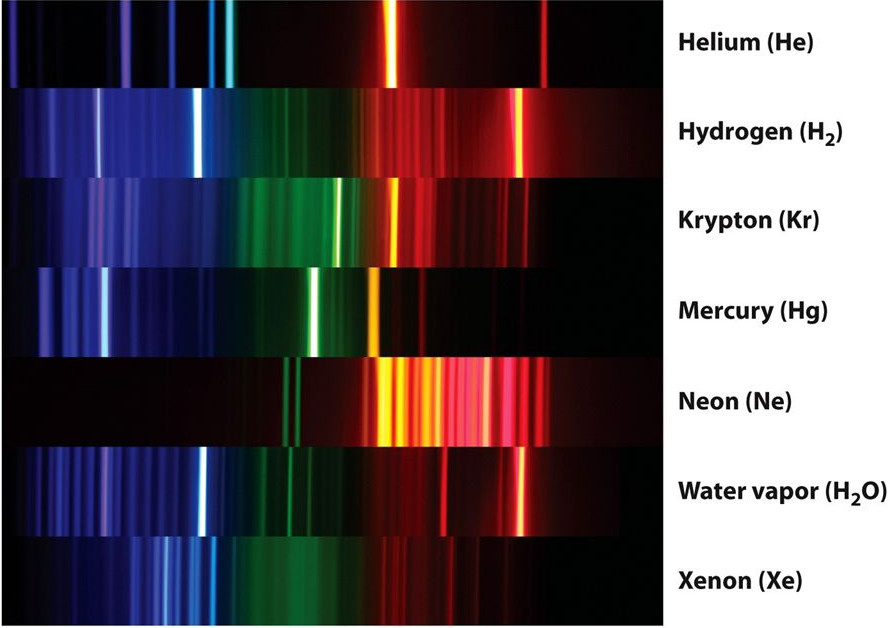
\includegraphics[width=.8\columnwidth]{img/spettriatomi.jpg}
\end{figure}
\end{frame}

\begin{frame}
\frametitle{Leggi sperimentali}
La legge sperimentale che permette di calcolare le $ \lambda $ emesse dall'idrogeno è la \emph{formula di Rydberg}:
\begin{center}
\colorbox{blue!30}{$ \dfrac{1}{\lambda} = R_H \left( \dfrac{1}{m^2} - \dfrac{1}{n^2} \right) $} ~~~~~~$ m,n \in \mathbb{N}, n > m $
\end{center}
$ R_H = 1,097 \times 10^7 \, m^{-1} $ = costante di Rydberg per H.\pause

~

\begin{itemize}
  \item $ m=1 $: serie spettrale di Lyman (nell'ultravioletto);\pause
  \item $ m=2 $: serie spettrale di Balmer (nel visibile);\pause
  \item $ m=3 $: serie spettrale di Paschen (nell'infrarosso).
\end{itemize}
\end{frame}



\begin{frame}
\frametitle{Perché?}
All'inizio del XX secolo non si capiva perché ogni elemento avesse uno specifico spettro.\pause

~

L'idea era che onde di qualunque lunghezza d'onda potessero far oscillare gli elettroni (essere assorbite) e che gli elettroni potessero oscillare con frequenza qualunque (ed emettere onde elettromagnetiche).\pause

~

La presenza di righe nette suggeriva che gli elettroni negli atomi potessero avere valori energetici discreti.
\end{frame}


\section{Elettroni}

\begin{frame}
\frametitle{Nascita e sviluppo del concetto di atomo}
\begin{columns}
\begin{column}{0.2\textwidth}
\visible<1->{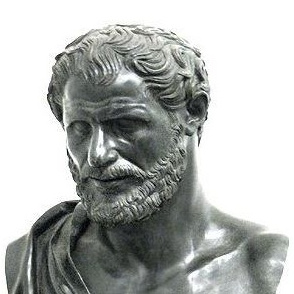
\includegraphics[width=\columnwidth]{img/democrito.jpg}}

\visible<2->{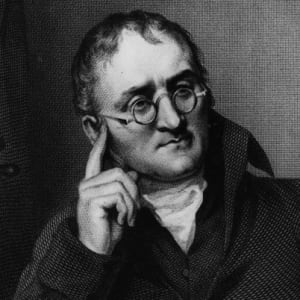
\includegraphics[width=\columnwidth]{img/dalton.jpg}}

\visible<3->{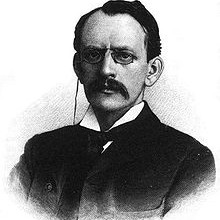
\includegraphics[width=\columnwidth]{img/thomson.jpg}}
\end{column}
\begin{column}{0.7\textwidth}
\begin{itemize}
\item<1-> Democrito ed Epicuro (V-III secolo a.C.) ipotizzano che la materia sia costituita \alert<1>{particelle indivisibili};
\item<2-> nel XIX secolo i nuovi sviluppi della \alert<2>{chimica} e della \alert<2>{termodinamica} possono essere spiegati mediante gli atomi (Dalton, Lavoisier, Boltzmann);
\item<3-> nel 1897 J.J.~Thomson dimostra che i raggi catodici sono formati da corpuscoli negativi, gli \alert<3>{elettroni}.
\end{itemize}
\visible<4>{Dopo la scoperta di Thomson, si rende necessario un \alert<4>{nuovo modello atomico} che tenga conto degli elettroni.}
\end{column}
\end{columns}
\end{frame}


\begin{frame}
\frametitle{Il modello di Dalton (1803)}
\begin{columns}
\begin{column}{0.2\textwidth}
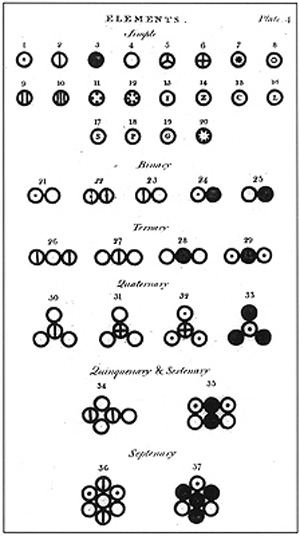
\includegraphics[width=\columnwidth]{img/atomidalton.jpg}
\end{column}
\begin{column}{0.7\textwidth}
Il modello di Dalton si basava sui seguenti principi:
\begin{itemize}
\item la materia è formata da particelle elementari indivisibili, gli atomi;
\item gli atomi di uno stesso elemento sono tutti uguali tra loro;
\item gli atomi di elementi diversi si combinano tra loro in rapporti di numeri interi e piccoli, originando i composti;
\item gli atomi non possono essere creati né distrutti;
\item gli atomi di un elemento non possono essere convertiti in atomi di altri elementi.
\end{itemize}
\end{column}
\end{columns}
\end{frame}





\begin{frame}
\frametitle{Il modello di Thomson (1904)}
Sapendo che la massa degli elettroni è molto piccola e che la materia è globalmente neutra, Thomson ipotizza che l'atomo sia costituito da una \alert<1>{sfera fluida di materia caricata positivamente in cui gli elettroni sono immersi}.\pause

~

\begin{columns}
\begin{column}{0.5\textwidth}
\emph{The atoms of the elements consist of a number of negatively electrified corpuscles enclosed in a sphere of uniform positive electrification.}
\vspace*{-1em}
\begin{flushright}
Thomson, 1904
\end{flushright}
\end{column}
\begin{column}{0.4\textwidth}
\begin{figure}
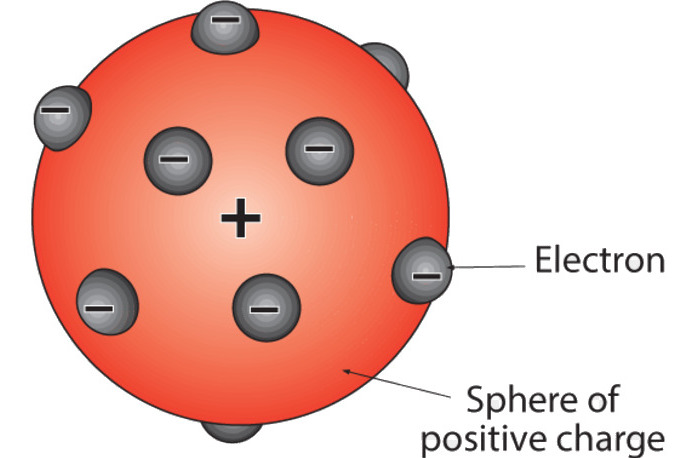
\includegraphics[width=\columnwidth]{img/atomothomson.jpg}
\end{figure}
\end{column}
\end{columns}

\end{frame}


\begin{frame}
\frametitle{L'esperimento di Millikan (1909)}
\begin{columns}
\begin{column}{0.55\textwidth}
\begin{figure}
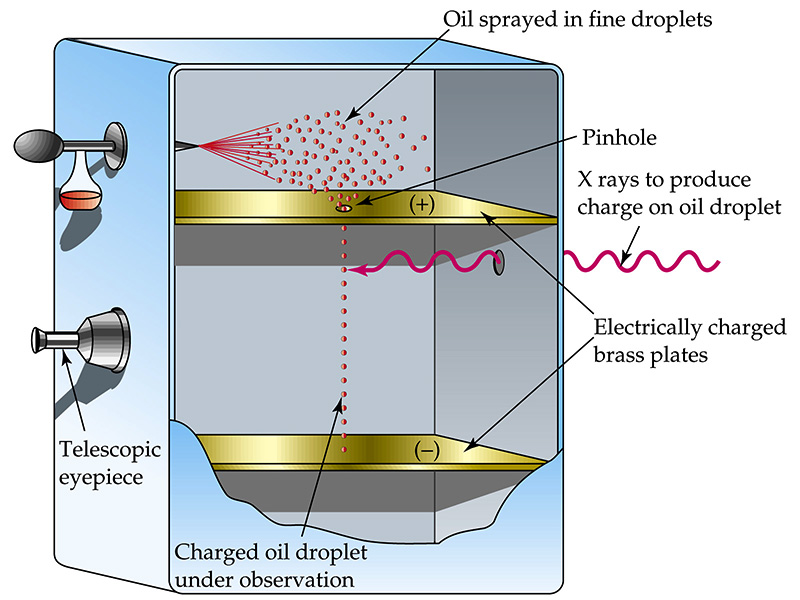
\includegraphics[width=\columnwidth]{img/millikanesp.jpg}
\end{figure}
\end{column}
\begin{column}{0.35\textwidth}
Permise di misurare la carica dell'elettrone con uno scarto dell'1\% rispetto al valore oggi accettato:
\begin{center}
\colorbox{blue!30}{$ e = 1,6021 \times 10^{-19} \, C $}
\end{center}
\end{column}
\end{columns}
\end{frame}


\section{Nucleo}

\begin{frame}
\frametitle{L'esperimento di Geiger e Marsden (1909)}
Ernest Rutherford, insieme ai collaboratori Hans Geiger e Ernest Marsden, sottopose il modello di Thomson ad esperimento, per testarne la validità.\pause

~

L'esperimento consisteva nel dirigere un \alert<2>{fascio di particelle $ \alpha $} (nuclei di elio, emessi da radon radioattivo) verso una lamina d'oro, metallo che può essere ridotto allo spessore di qualche migliaio di atomi.\pause

~

Ci si aspettava che le particelle $ \alpha $, $ 10^4 $ volte più pesanti degli elettroni, avrebbero \alert<3>{attraversato la lamina d'oro con deviazioni minime}, dovute alla debole interazione con gli elettroni.
\end{frame}




\begin{frame}
\frametitle{Schema dell'esperimento e risultati}
\begin{figure}
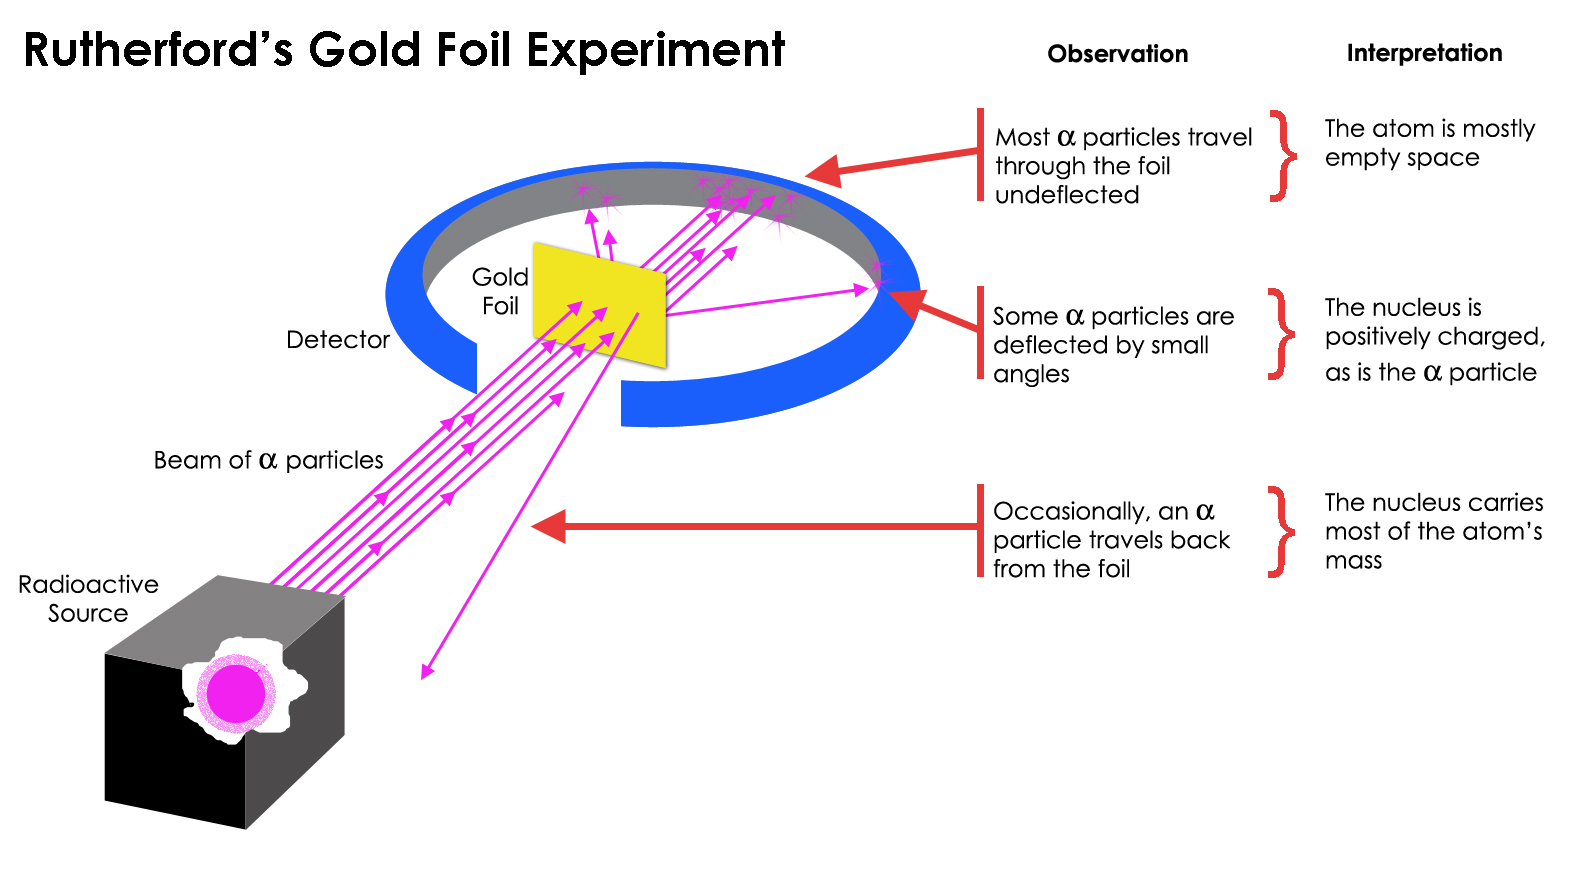
\includegraphics[width=\columnwidth]{img/esperimentorutherford.jpg}
\end{figure}
\end{frame}



\begin{frame}
\frametitle{Nelle parole di Rutherford}
\emph{It was quite the most incredible event that has ever happened to me in my life. It was almost as incredible as if you fired a 15-inch shell at a piece of tissue paper and it came back and hit you.

~~On consideration, I realized that this scattering backward must be the result of a single collision, and when I made calculations I saw that it was impossible to get anything of that order of magnitude unless you took a system in which the greater part of the mass of the atom was concentrated in a minute nucleus.

~~It was then that I had the idea of an atom with a minute massive centre, carrying a charge.}
\begin{flushright}
Ernest Rutherford, 1934
\end{flushright}
\end{frame}


\begin{frame}
\frametitle{Il modello planetario (1911)}
Il modello proposto da Rutherford prevede che:
\begin{itemize}
  \item \alert<1>{la maggior parte della massa dell'atomo è concentrata nel nucleo} (un nucleone è migliaia di volte più pesante di un elettrone);\pause
  \item \alert<2>{la maggior parte del volume occupato dall'atomo è vuoto} (per l'oro, il raggio del nucleo è nell'ordine dei $ 10^{-14} \, m $, quello della nuvola elettronica $ 10^{-10} \, m $).
\end{itemize}
\begin{figure}
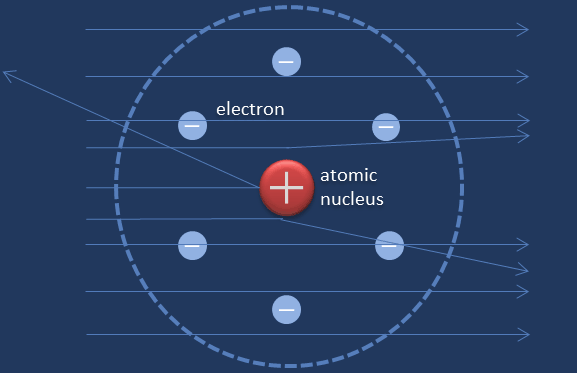
\includegraphics[width=.4\columnwidth]{img/atomorutherford.png}
\end{figure}
\end{frame}



\begin{frame}
\frametitle{Problemi del modello planetario}
Il modello planetario di Rutherford non poteva tuttavia essere corretto. Infatti:
\begin{itemize}
  \item se un elettrone percorre un'orbita circolare, esso subisce un'accelerazione centripeta;\pause
  \item elettroni accelerati emettono onde elettromagnetiche, perdendo energia;\pause
  \item se viene persa energia, il raggio dell'orbita diminuisce;\pause
  \item l'elettrone dovrebbe ``cadere'' sul nucleo in breve tempo ($ 10^{-7} \, s $).
\end{itemize}
\end{frame}

\section{Bohr}

\begin{frame}
\frametitle{Le ipotesi di Bohr (1912)}
\begin{columns}
\begin{column}{0.2\textwidth}
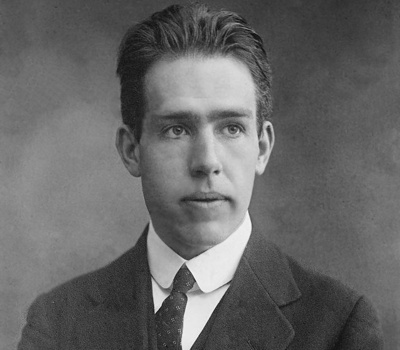
\includegraphics[width=\columnwidth]{img/bohr.jpg}
\end{column}
\begin{column}{0.7\textwidth}
Neils Bohr, allievo di Rutherford, propose un modello per cui:
\begin{itemize}
\item il raggio delle orbite degli elettroni attorno al nucleo può avere soltanto un certo insieme di valori permessi;\pause
\item quando l’elettrone percorre una di queste orbite (dotate di un'energia totale ben definita) non irraggia.
\end{itemize}
\end{column}
\end{columns}
\end{frame}


\begin{frame}
\frametitle{Quantizzazione dell'orbita (1)}
Dalle sue assunzioni, Bohr poté calcolare il raggio delle orbite permesse agli elettroni dell'atomo di idrogeno, secondo la relazione:
\begin{center}
$ 2 \pi r_n p_n  = nh $
\end{center}
\begin{itemize}
  \item $ n $ = intero positivo, numero quantico principale;
  \item $ r_n $ = raggio dell'orbita numero $ n $;
  \item $ p_n $ = quantità di moto dell'orbita $ n $.
\end{itemize}
\end{frame}


\begin{frame}
\frametitle{Quantizzazione dell'orbita (2)}
\begin{columns}
\begin{column}{0.6\textwidth}
Ipotizzando ora che la forza di Coulomb agisca come forza centripeta, possiamo ottenere:
\begin{center}
\colorbox{blue!30}{$ r(n) = \dfrac{\varepsilon_0 h^2}{\pi m_e e^2} n^2 = (5,29 \times 10^{-11}) n^2  $}
\end{center}
\end{column}
\begin{column}{0.4\textwidth}
\begin{figure}
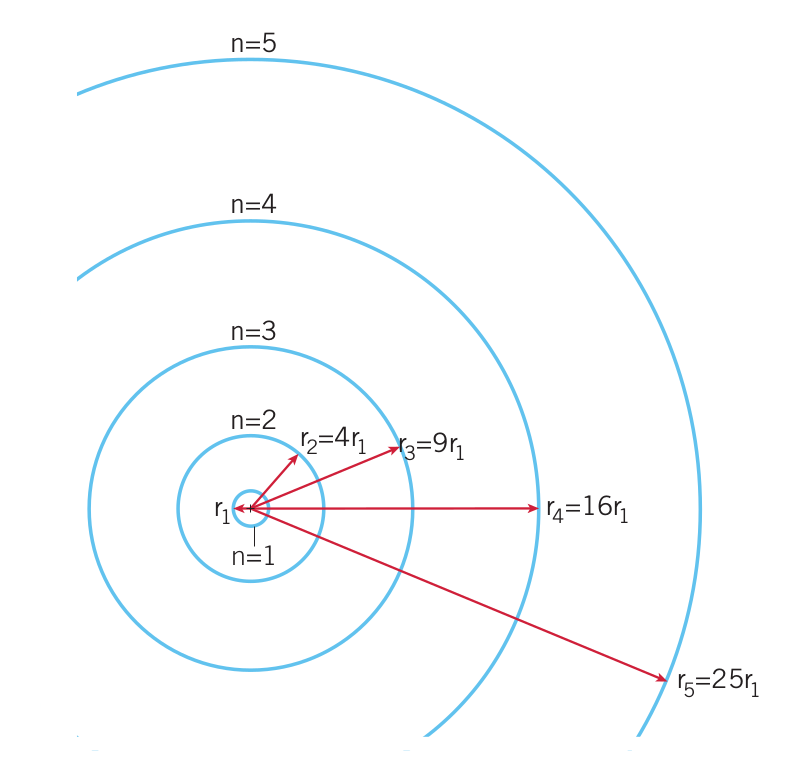
\includegraphics[width=\columnwidth]{img/orbite.png}
\end{figure}

~
\end{column}
\end{columns}\pause
Possiamo inoltre calcolare l'energia associata ad ogni orbita:
\begin{center}
\colorbox{blue!30}{$ E(n) = - \dfrac{m_e e^4}{8\varepsilon_0^2 h^2 n^2} = - \dfrac{13,6 \, eV}{n^2} $}
\end{center}
\end{frame}


%dimostrazione?


\begin{frame}
\frametitle{Emissione di fotoni (1)}
Lo stato dell'elettrone a cui corrisponde l'orbita a minore energia è detto \alert<1>{stato fondamentale}.\pause

~

Se l'elettrone riceve energia sufficiente (ad esempio mediante onde elettromagnetiche), può passare ad uno \alert<2>{stato eccitato}.\pause

~

Secondo Bohr:

\begin{block}{Emissione di fotoni}
quando un elettrone passa da un'orbita permessa ad energia maggiore ad una ad energia minore, emette un fotone.
\end{block}
\end{frame}




\begin{frame}
\frametitle{Emissione di fotoni (1)}
\begin{figure}
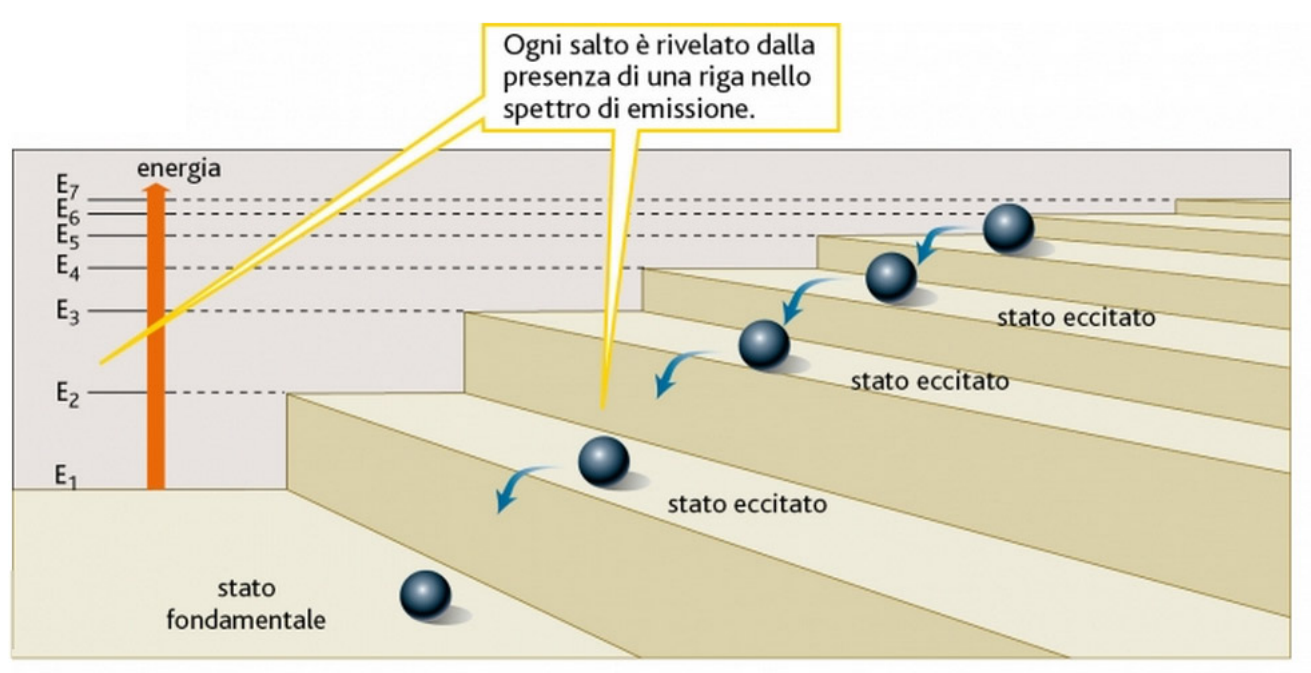
\includegraphics[width=\columnwidth]{img/emissionefotoni1.png}
\end{figure}
\end{frame}

\begin{frame}
\frametitle{Emissione di fotoni (2)}
Immaginiamo un fotone eccitato sull'orbita di numero quantico $ n $.\pause

~

Tale orbita è instabile, e l'elettrone si sposterà su un'orbita a energia minore di numero quantico $ m < n $.\pause

~

L'energia del fotone emesso durante il passaggio sarà la differenza di energia tra le due orbite dell'elettrone:
\begin{center}
$ E = E(n) - E(m) $
\end{center}
\end{frame}

\begin{frame}
\frametitle{Emissione di fotoni (3)}
Se l'energia del fotone è legata alla sua frequenza da $ E = hf $, otteniamo:
\begin{center}
$ f = \dfrac{E(n) - E(m)}{h} $~~~$ \Longrightarrow  $~~~$ f = \dfrac{m_e e^4}{8\varepsilon_0^2 h^3} \left( \dfrac{1}{m^2} - \dfrac{1}{n^2} \right) $
\end{center}\pause
Ricordando che $ f = \dfrac{c}{\lambda} $ otteniamo:
\begin{center}
$ \dfrac{1}{\lambda} = \alert<3>{\dfrac{m_e e^4}{8 c \varepsilon_0^2 h^3}} \left( \dfrac{1}{m^2} - \dfrac{1}{n^2} \right) $
\end{center}\pause
Tale formula permette di calcolare per via teorica la \alert<3>{costante di Rydberg} per l'atomo di idrogeno, spiegando pertanto i risultati sperimentali.
\end{frame}


\begin{frame}
\frametitle{La serie spettrale di Balmer}
\begin{figure}
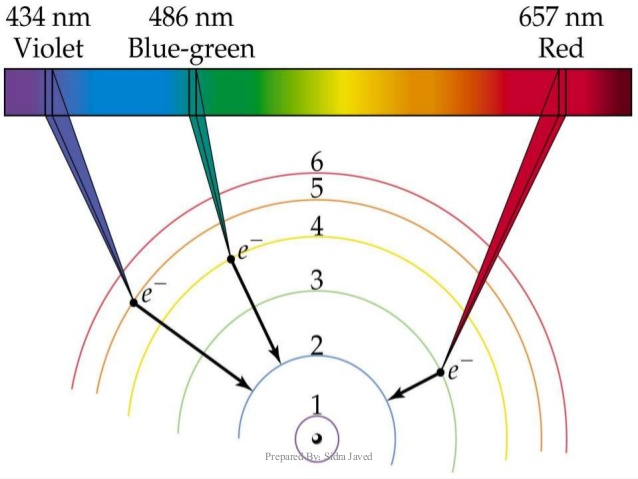
\includegraphics[width=.7\columnwidth]{img/balmeridrogeno.jpg}
\end{figure}
\end{frame}




\begin{frame}
\frametitle{Le altre serie spettrali}
\begin{figure}
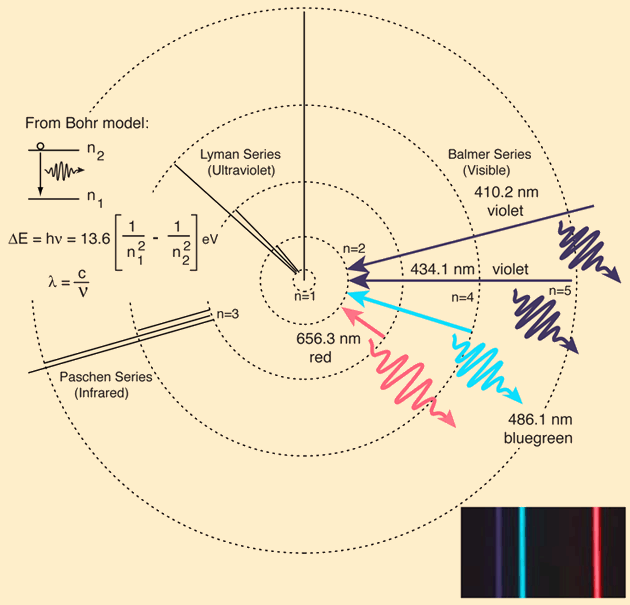
\includegraphics[width=.7\columnwidth]{img/emissionefotoni2.png}
\end{figure}
\end{frame}

%\section{Franck e Hertz}



\end{document}
